% Options for packages loaded elsewhere
\PassOptionsToPackage{unicode}{hyperref}
\PassOptionsToPackage{hyphens}{url}
%
\documentclass[
  ignorenonframetext,
]{beamer}
\usepackage{pgfpages}
\setbeamertemplate{caption}[numbered]
\setbeamertemplate{caption label separator}{: }
\setbeamercolor{caption name}{fg=normal text.fg}
\beamertemplatenavigationsymbolsempty
% Prevent slide breaks in the middle of a paragraph
\widowpenalties 1 10000
\raggedbottom
\setbeamertemplate{part page}{
  \centering
  \begin{beamercolorbox}[sep=16pt,center]{part title}
    \usebeamerfont{part title}\insertpart\par
  \end{beamercolorbox}
}
\setbeamertemplate{section page}{
  \centering
  \begin{beamercolorbox}[sep=12pt,center]{part title}
    \usebeamerfont{section title}\insertsection\par
  \end{beamercolorbox}
}
\setbeamertemplate{subsection page}{
  \centering
  \begin{beamercolorbox}[sep=8pt,center]{part title}
    \usebeamerfont{subsection title}\insertsubsection\par
  \end{beamercolorbox}
}
\AtBeginPart{
  \frame{\partpage}
}
\AtBeginSection{
  \ifbibliography
  \else
    \frame{\sectionpage}
  \fi
}
\AtBeginSubsection{
  \frame{\subsectionpage}
}
\usepackage{amsmath,amssymb}
\usepackage{lmodern}
\usepackage{ifxetex,ifluatex}
\ifnum 0\ifxetex 1\fi\ifluatex 1\fi=0 % if pdftex
  \usepackage[T1]{fontenc}
  \usepackage[utf8]{inputenc}
  \usepackage{textcomp} % provide euro and other symbols
\else % if luatex or xetex
  \usepackage{unicode-math}
  \defaultfontfeatures{Scale=MatchLowercase}
  \defaultfontfeatures[\rmfamily]{Ligatures=TeX,Scale=1}
  \setmainfont[BoldFont = SF Pro Rounded Semibold]{SF Pro Rounded}
  \setmathfont[]{STIX Two Math}
\fi
\usefonttheme{serif} % use mainfont rather than sansfont for slide text
% Use upquote if available, for straight quotes in verbatim environments
\IfFileExists{upquote.sty}{\usepackage{upquote}}{}
\IfFileExists{microtype.sty}{% use microtype if available
  \usepackage[]{microtype}
  \UseMicrotypeSet[protrusion]{basicmath} % disable protrusion for tt fonts
}{}
\makeatletter
\@ifundefined{KOMAClassName}{% if non-KOMA class
  \IfFileExists{parskip.sty}{%
    \usepackage{parskip}
  }{% else
    \setlength{\parindent}{0pt}
    \setlength{\parskip}{6pt plus 2pt minus 1pt}}
}{% if KOMA class
  \KOMAoptions{parskip=half}}
\makeatother
\usepackage{xcolor}
\IfFileExists{xurl.sty}{\usepackage{xurl}}{} % add URL line breaks if available
\IfFileExists{bookmark.sty}{\usepackage{bookmark}}{\usepackage{hyperref}}
\hypersetup{
  pdftitle={444 Lecture 4.5 - Subgame Perfect Equilibrium},
  pdfauthor={Brian Weatherson},
  hidelinks,
  pdfcreator={LaTeX via pandoc}}
\urlstyle{same} % disable monospaced font for URLs
\newif\ifbibliography
\usepackage{graphicx}
\makeatletter
\def\maxwidth{\ifdim\Gin@nat@width>\linewidth\linewidth\else\Gin@nat@width\fi}
\def\maxheight{\ifdim\Gin@nat@height>\textheight\textheight\else\Gin@nat@height\fi}
\makeatother
% Scale images if necessary, so that they will not overflow the page
% margins by default, and it is still possible to overwrite the defaults
% using explicit options in \includegraphics[width, height, ...]{}
\setkeys{Gin}{width=\maxwidth,height=\maxheight,keepaspectratio}
% Set default figure placement to htbp
\makeatletter
\def\fps@figure{htbp}
\makeatother
\setlength{\emergencystretch}{3em} % prevent overfull lines
\providecommand{\tightlist}{%
  \setlength{\itemsep}{0pt}\setlength{\parskip}{0pt}}
\setcounter{secnumdepth}{-\maxdimen} % remove section numbering
\let\Tiny=\tiny

 \setbeamertemplate{navigation symbols}{} 

% \usetheme{Madrid}
 \usetheme[numbering=none, progressbar=foot]{metropolis}
 \usecolortheme{wolverine}
 \usepackage{color}
 \usepackage{MnSymbol}
% \usepackage{movie15}

\usepackage{amssymb}% http://ctan.org/pkg/amssymb
\usepackage{pifont}% http://ctan.org/pkg/pifont
\newcommand{\cmark}{\ding{51}}%
\newcommand{\xmark}{\ding{55}}%

\DeclareSymbolFont{symbolsC}{U}{txsyc}{m}{n}
\DeclareMathSymbol{\boxright}{\mathrel}{symbolsC}{128}
\DeclareMathAlphabet{\mathpzc}{OT1}{pzc}{m}{it}

\setlength{\parskip}{1ex plus 0.5ex minus 0.2ex}

\AtBeginSection[]
{
\begin{frame}
	\Huge{\color{darkblue} \insertsection}
\end{frame}
}

\renewenvironment*{quote}	
	{\list{}{\rightmargin   \leftmargin} \item } 	
	{\endlist }

\definecolor{darkgreen}{rgb}{0,0.7,0}
\definecolor{darkblue}{rgb}{0,0,0.8}

\usepackage[italic]{mathastext}
\usepackage{nicefrac}

\setbeamertemplate{caption}{\raggedright\insertcaption}

%\def\toprule{}
%\def\bottomrule{}
%\def\midrule{}
\usepackage{etoolbox}
\AfterEndEnvironment{description}{\vspace{9pt}}
\AfterEndEnvironment{oltableau}{\vspace{9pt}}
\BeforeBeginEnvironment{oltableau}{\vspace{9pt}}
\AfterEndEnvironment{center}{\vspace{9pt}}
\BeforeBeginEnvironment{tabular}{\vspace{9pt}}
\AfterEndEnvironment{longtable}{\vspace{-6pt}}
\usepackage{booktabs}
\usepackage{longtable}
\usepackage{array}
\usepackage{multirow}
\usepackage{wrapfig}
\usepackage{float}
\usepackage{colortbl}
\usepackage{pdflscape}
\usepackage{tabu}
\usepackage{threeparttable} 
\usepackage{threeparttablex} 
\usepackage[normalem]{ulem} 
\usepackage{makecell}
\usepackage{xcolor}
\usepackage{ulem}

\setlength\heavyrulewidth{0ex}
\setlength\lightrulewidth{0.08ex}

\aboverulesep=0ex
\belowrulesep=0ex
\renewcommand{\arraystretch}{1.2}
\ifluatex
  \usepackage{selnolig}  % disable illegal ligatures
\fi

\title{444 Lecture 4.5 - Subgame Perfect Equilibrium}
\author{Brian Weatherson}
\date{}

\begin{document}
\frame{\titlepage}

\begin{frame}{Plan}
\protect\hypertarget{plan}{}
To describe the notion of subgame perfect equilibrium.
\end{frame}

\begin{frame}{Reading}
\protect\hypertarget{reading}{}
Bonanno, section 4.4.
\end{frame}

\begin{frame}{Definition}
\protect\hypertarget{definition}{}
A set of strategies for each of the players is a subgame perfect
equilibrium if and only if

\begin{itemize}
\tightlist
\item
  The set forms a Nash equilibrium.
\item
  In every subgame, the set forms a Nash equilibrium.
\end{itemize}
\end{frame}

\begin{frame}{Subgame Perfect and Nash}
\protect\hypertarget{subgame-perfect-and-nash}{}
The second clause is non-trivial.

\begin{itemize}
\tightlist
\item
  It rules out players doing certain kinds of odd things at nodes that
  are not reached.
\item
  At subgame perfect equilibrium, each player's strategies make sense
  given the other player's strategies, and they are disposed to keep
  making sense under different assumptions about what they might do.
\end{itemize}
\end{frame}

\begin{frame}{Finding Subgame Perfect Equilibrium}
\protect\hypertarget{finding-subgame-perfect-equilibrium}{}
\begin{itemize}
\tightlist
\item
  Find the minimal subgames.
\item
  Act as if the initial node of that subgame is a terminal node, with
  its payouts being the equilibrium payouts of the subgame.
\item
  If there are multiple equilibria, duplicate the tree enough times to
  cover each of them - you'll have multiple subgame perfect equilibria.
\item
  Repeat until you've covered the whole tree.
\end{itemize}
\end{frame}

\begin{frame}
\begin{figure}
\centering
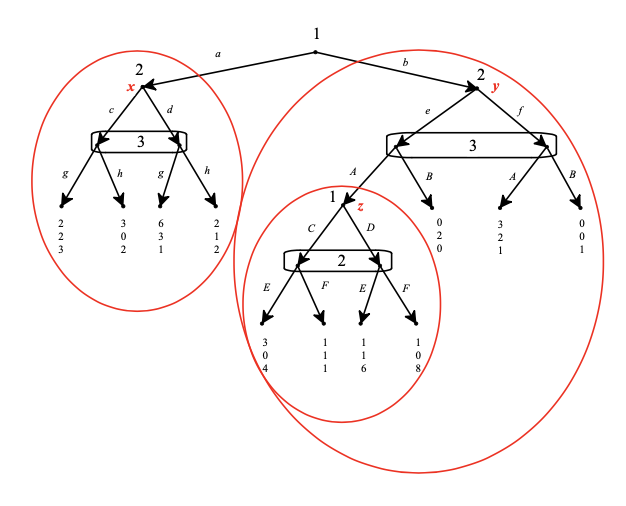
\includegraphics[width=\textwidth,height=0.8\textheight]{images/04_03.png}
\caption{The large game}
\end{figure}
\end{frame}

\begin{frame}
\begin{figure}
\centering
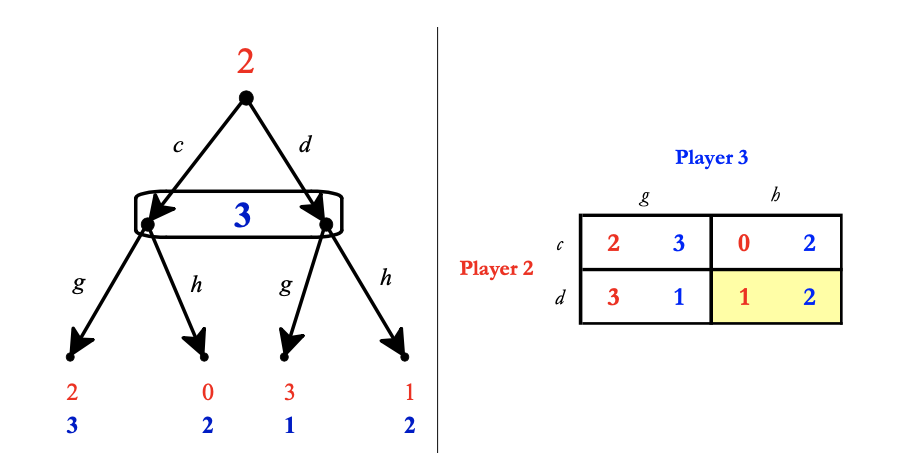
\includegraphics[width=\textwidth,height=0.8\textheight]{images/04_04.png}
\caption{The left subgame}
\end{figure}
\end{frame}

\begin{frame}
\begin{figure}
\centering
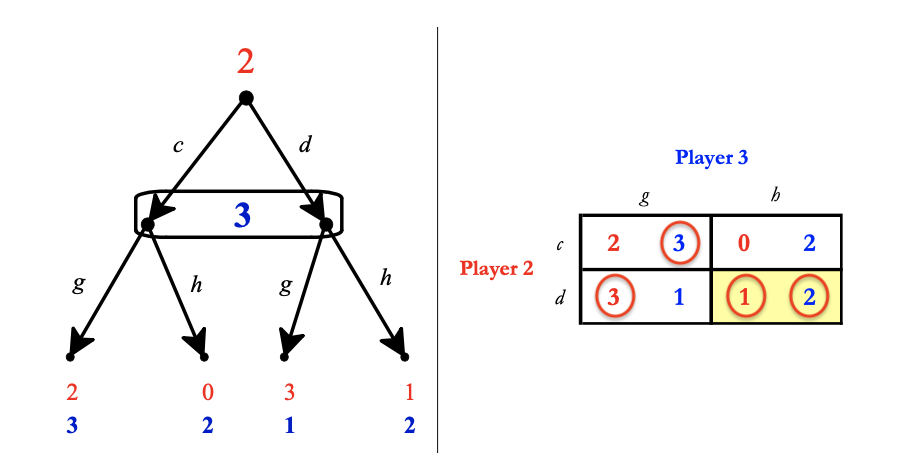
\includegraphics[width=\textwidth,height=0.8\textheight]{images/04_05.png}
\caption{The left subgame with labeled best responses}
\end{figure}
\end{frame}

\begin{frame}
\begin{figure}
\centering
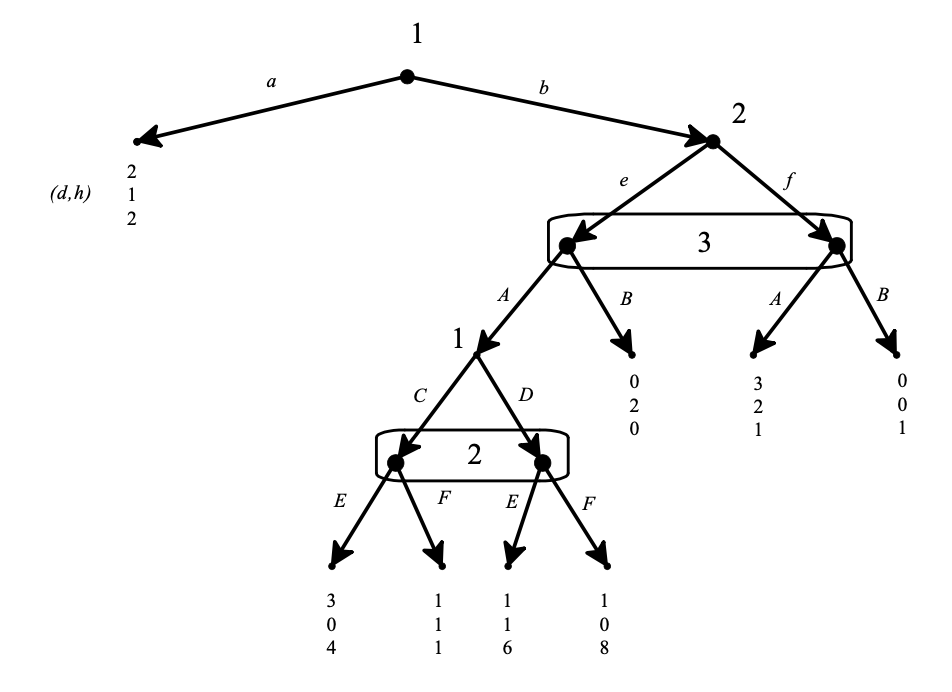
\includegraphics[width=\textwidth,height=0.8\textheight]{images/04_06.png}
\caption{The big game with reduced left subgame}
\end{figure}
\end{frame}

\begin{frame}
\begin{figure}
\centering
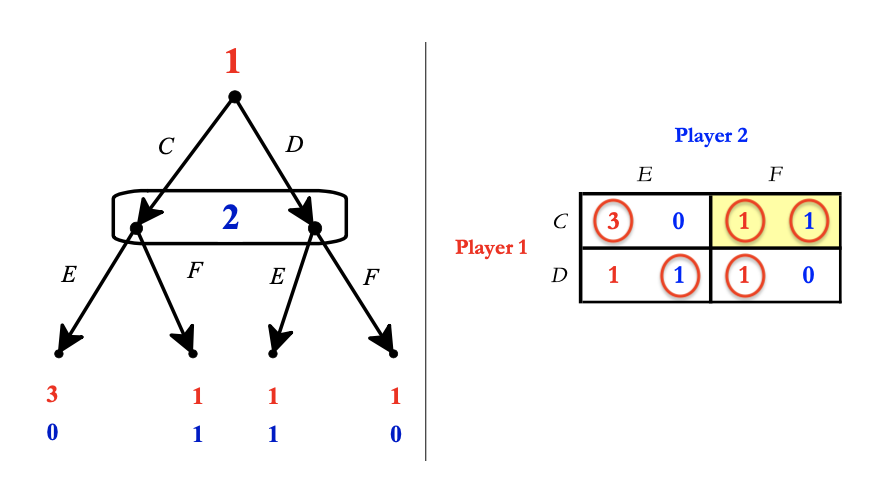
\includegraphics[width=\textwidth,height=0.8\textheight]{images/04_07.png}
\caption{The middle subgame with labeled best responses}
\end{figure}
\end{frame}

\begin{frame}
\begin{figure}
\centering
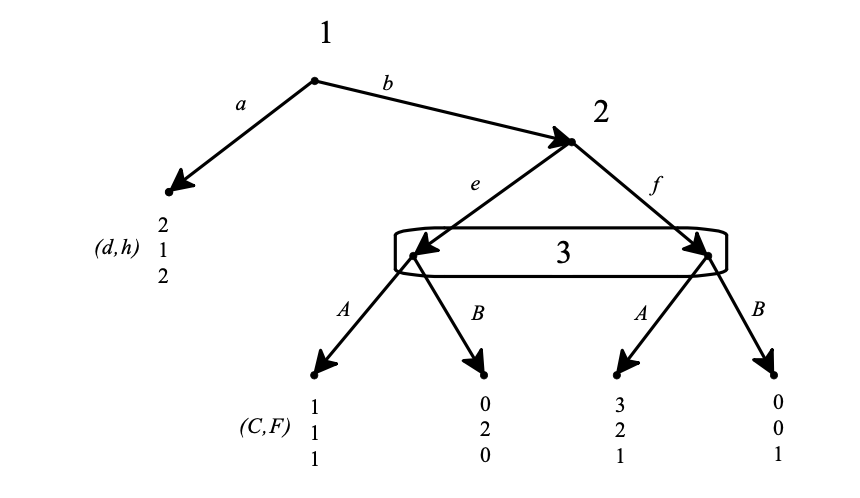
\includegraphics[width=\textwidth,height=0.8\textheight]{images/04_08.png}
\caption{The big game with reduced middle subgame}
\end{figure}
\end{frame}

\begin{frame}{The right subgame}
\protect\hypertarget{the-right-subgame}{}
\begin{table}[!h]
\centering
\begin{tabular}[t]{>{}r|cc}
\toprule
 & A & B\\
\midrule
e & 1, 1 & 2, 0\\
f & 2, 1 & 0, 1\\
\bottomrule
\end{tabular}
\end{table}

\begin{itemize}
\tightlist
\item
  Player 2 is row
\item
  Player 3 is column
\item
  Player 1 is ignored, because they have no moves
\end{itemize}
\end{frame}

\begin{frame}{The right subgame with labeled best responses}
\protect\hypertarget{the-right-subgame-with-labeled-best-responses}{}
\begin{table}[!h]
\centering
\begin{tabular}[t]{>{}r|cc}
\toprule
 & A & B\\
\midrule
e & 1, \fbox{1} & \fbox{2}, 0\\
f & \fbox{2}, \fbox{1} & 0, \fbox{1}\\
\bottomrule
\end{tabular}
\end{table}
\end{frame}

\begin{frame}
\begin{figure}
\centering
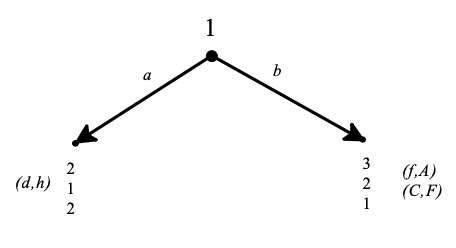
\includegraphics[width=\textwidth,height=0.7\textheight]{images/04_09.png}
\caption{The big game with reduced right subgame}
\end{figure}

\begin{itemize}
\tightlist
\item
  Only Nash equilibrium is Player 1 plays \(b\).
\end{itemize}
\end{frame}

\begin{frame}{Summary}
\protect\hypertarget{summary}{}
So the subgame perfect equilibrium is:

\begin{itemize}
\tightlist
\item
  Player 1 plays \(b, C\).
\item
  Player 2 plays \(d, f, F\).
\item
  Player 3 plays \(h, A\).
\end{itemize}

And the payouts are reverse order of their names: 3, 2, 1.
\end{frame}

\begin{frame}{For Next Time}
\protect\hypertarget{for-next-time}{}
We will start looking at games with cardinal utility.
\end{frame}

\end{document}
